%%%%%%%%%%%%%%%%%%%%%%%%%%%%%%%%%%%%%%%%%%%%%%%%%%%%%%%%%%%%%%%%%%%%%%
% LaTeX Example: Project Report
%
% Source: http://www.howtotex.com
%
% Feel free to distribute this example, but please keep the referral
% to howtotex.com
% Date: March 2011 
% 
%%%%%%%%%%%%%%%%%%%%%%%%%%%%%%%%%%%%%%%%%%%%%%%%%%%%%%%%%%%%%%%%%%%%%%
% How to use writeLaTeX: 
%
% You edit the source code here on the left, and the preview on the
% right shows you the result within a few seconds.
%
% Bookmark this page and share the URL with your co-authors. They can
% edit at the same time!
%
% You can upload figures, bibliographies, custom classes and
% styles using the files menu.
%
% If you're new to LaTeX, the wikibook is a great place to start:
% http://en.wikibooks.org/wiki/LaTeX
%
%%%%%%%%%%%%%%%%%%%%%%%%%%%%%%%%%%%%%%%%%%%%%%%%%%%%%%%%%%%%%%%%%%%%%%
% Edit the title below to update the display in My Documents
%\title{Project Report}
%
%%% Preamble
\documentclass[paper=a4, fontsize=11pt]{scrartcl}
\usepackage[T1]{fontenc}
\usepackage{fourier}
\usepackage{tabularx}

\usepackage{graphicx}

\usepackage[english]{babel}															% English language/hyphenation
\usepackage[protrusion=true,expansion=true]{microtype}	
\usepackage{amsmath,amsfonts,amsthm} % Math packages

\usepackage{url}
\usepackage[hang, small,labelfont=bf,up,textfont=it,up]{caption}


%%% Custom sectioning
\usepackage{sectsty}
\allsectionsfont{\centering \normalfont\scshape}
\usepackage{float}

%%% Custom headers/footers (fancyhdr package)
\usepackage{fancyhdr}
\pagestyle{fancyplain}
\fancyhead{}											% No page header
\fancyfoot[L]{}											% Empty 
\fancyfoot[C]{}											% Empty
\fancyfoot[R]{\thepage}									% Pagenumbering
\renewcommand{\headrulewidth}{0pt}			% Remove header underlines
\renewcommand{\footrulewidth}{0pt}				% Remove footer underlines
\setlength{\headheight}{13.6pt}


%%% Equation and float numbering
\numberwithin{equation}{section}		% Equationnumbering: section.eq#
\numberwithin{figure}{section}			% Figurenumbering: section.fig#
\numberwithin{table}{section}				% Tablenumbering: section.tab#


%%% Maketitle metadata
\newcommand{\horrule}[1]{\rule{\linewidth}{#1}} 	% Horizontal rule

\title{
		%\vspace{-1in} 	
		\usefont{OT1}{bch}{b}{n}
		\normalfont \normalsize \textsc{Thompson Rivers University} \\ [25pt]
		
\includegraphics[width=0.1\linewidth]{tru}
		\horrule{0.5pt} \\[0.2cm]
		\huge 9XTend RF Module Wireless Device Report \\
		\horrule{2pt} \\[0.005cm]
}
\author{
		\normalfont 								\normalsize
        Jerin Roberts\\[-3pt]		\normalsize
        \today
}
\date{}


%%% Begin document
\begin{document}
\maketitle

\section{Introduction}

The 9Xtend RF module is a wireless device capable of transmitting and receiving data over long ranges. The 9Xtend module was designed to provide an easy to use platform that has the ability to deliver reliable data between remote devices. The module transfers a standard asynchronous serial data stream while operating within the ISM 900 MHz band range.

\begin{figure}[h!]
\centering
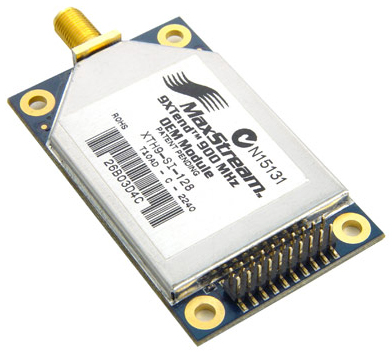
\includegraphics[width=0.5\linewidth]{9X}
\caption{The 9Xtend RF module used for wireless data transmission}
\label{x9}
\end{figure}
This is a range reserved for industrial, scientific and medical use (ISM) and therefore doesn't require significant licensing or documentation for operation. Delivering a variable output of up to 1W the 9Xtend has many indoor and outdoor applications.

\section{Networking}

The module is able to attain reliable outdoor data transfer within a 22km range with a standard dipole antenna, line of sight. With a high gain antenna this could easily be extended to 64km line of sight. The module broadcasts on range of frequencies from 902-928MHz. To attain reliable connections the module employs the use of Frequency-Hopping Spread Spectrum (FHSS) which is a method of transmitting radio signals by rapidly switching a carrier among many frequency channels using a random sequence known to both transmitter and receiver. A spread spectrum offers a number of advantages over conventional transmission methods. Spread-spectrum signals are highly resistant to narrowband interference.

\begin{figure}[h!]
\centering
\includegraphics[width=0.25\linewidth]{fsk}
\caption{Displays the use of frequency shift keying modulation to encode information onto a carrier signal \cite{picfsk}}
\label{fsk}
\end{figure}
During the process of re-collecting or capturing the spread of signals sent by the transmitter, the interfering signal is spread out among the signals and when the transmitted signals are recombined the net effect of the interfering signal on the newly combined signal is negligible. Therefore this method increases reliability against interfering sources that typically emanate from radio stations, TV stations or cell phones. Spread-spectrum signals are also difficult to intercept. A spread-spectrum signal may simply appear as an increase in the background noise to a narrowband receiver and unless the algorithm for the signal switching is known the interceptor will have little to no luck locking on the transmission. For information encoding onto the carrier the module uses frequency shift keying (FSK) modulation. FSK is a frequency modulation scheme in which digital information is transmitted through discrete frequency changes to the carrier wave. An visual interpretation of this is displayed in figure \ref{fsk}.
\section{Pin Layout}

\begin{figure}[H]
\centering
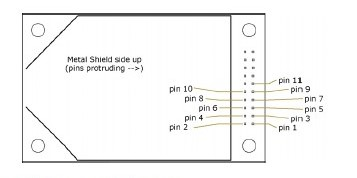
\includegraphics[width=0.5\linewidth]{spec1}
\caption{Displays the pin configuration for 9Xtend module \cite{man}}
\label{spec1}
\end{figure}



\begin{table}[H]
\begin{tabularx}{\textwidth}{ |X|X|X|X| }
\hline
Pin Number & Mnemonic & Function & Must Connect? \\ 
\hline
1 & Gnd & Ground & Y \\
\hline
2 & VCC & Power 2.8-5.5VDC & Y\\
\hline
5 & DI & Data IN & Y \\
\hline
6 & DO & Data OUT & Y \\
\hline
7 & SHDN & Shut-Down Mode (5uA) & Y \\
\hline
\end{tabularx}
\caption{This table displays the pins used for wireless transmission (For use with Figure \ref{spec1}) }
\label{spec2}
\end{table}





\section{Serial Communication}
The Xtend module can connected to a host device through a TTL-level asynchronous serial port \cite{man}. This enables the module to communicate with any Universal Asynchronous Transmitter or Receiver (UART) compatible device or through a level translator to any serial device. Devices with UART compatibility can connect directly to the module for communication as displayed in figure \ref{uartf}. 

\begin{figure}[h!]
\centering
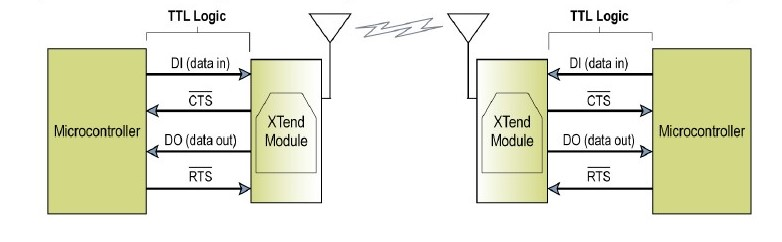
\includegraphics[width=0.8\linewidth]{uartf}
\caption{ Displays the system flow in a UART interfaced environment \cite{man}}
\label{uartf}
\end{figure}

The UART takes bytes of data and transmits the individual bits in a sequential fashion. The receiver contains a second UART that essentially re-assembles the bits into complete bytes. In order for the module to understand the incoming data it needs to be in a specific format (UART protocol) which is schematically shown in figure \ref{uartb}.
\begin{figure}[h!]
\centering
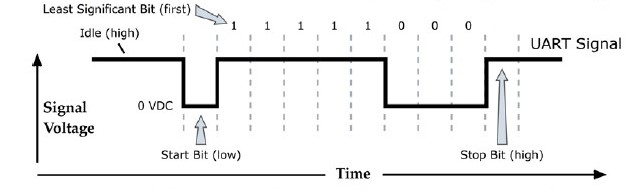
\includegraphics[width=0.8\linewidth]{uartb}
\caption{ Displays the format of a tyical UART data package \cite{man}}
\label{uartb}
\end{figure}

This can enter the module in UART format through pin 5 as an asynchronous serial signal. Each data package consists of a start bit, 8 data bits and then a stop bit. The signal should idle high when no data is being transmitted. Then a low pulse in the signal indicates a start bit, which will then be followed by the 8 bit data pulse beginning with the least significant bit. As usual a high signal represents a 1 and a low indicates a 0. Once 8 bits has been detected the signal is returned high to indicate a stop bit. From here the signal will idle high until another start bit initiates the process all over again. When the module is not transmitting or receiving it is in Idle mode.
\section{Flow Control}

\begin{figure}[H]
\centering
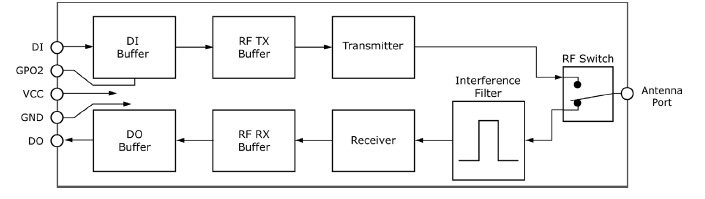
\includegraphics[width=0.9\linewidth]{flow}
\caption{ Displays the internal data flow diagram \cite{man}}
\label{flow}
\end{figure}
For data transmission the module uses data-IN buffer flow control. When serial data enters the input (pin 5) the data is initially stored to the DI buffer. RF transmission begins either after RB bytes (packatization threshold) has been received by the UART or a significant silence has been observed and a timeout function initializes transmission (i.e. data segment ends). Once one of these are satisfied the module attempts to initialize an RF connection. If the module is in the process of receiving data the serial is stored in the modules DI buffer (Fig.\ref{flow}). The DI buffer can store up to 2KB of information before overflow occurs. Unless flow control functions are initiated at this point data loss will occur. There are two cases in which the buffer may overflow. The first is if the serial rate from the host exceeds the RF rate of the module. The second is if the module is receiving a continuous stream of RF data, such that it never has the chance to transmit before the DI buffer overflows. By sending packages smaller than the DI buffer size and interfacing at a lower baud rate than the RF rate, then the earlier discussed scenarios can be avoided data loss won't occur using default flow control settings. 
Similarly when RF data is received the data enters the DO buffer and is sent out when a silence is detected. If none is detected the DI buffer will overflow and data loss will occur. This again can be prevented by the limits discussed previously in the section. Once a silence is detected the DO buffer sends data in a UART format to the host device. If should be noted that the input (pin 5) needs to be set high in order to receive data from the output (pin 6).


\section{Arduino Shield}

The 9Xtend is generally a stand-alone wireless communicator, however it still requires a device to organize and send data in the correct UART protocol. For the purposes of high altitude ballooning an Arduino platform was chosen to interface with the RF modules. In order for the module to successfully send and receive data to and from the Arduino it required a custom built physical interface known as an Arduino shield. 
\begin{figure}[H]
\centering
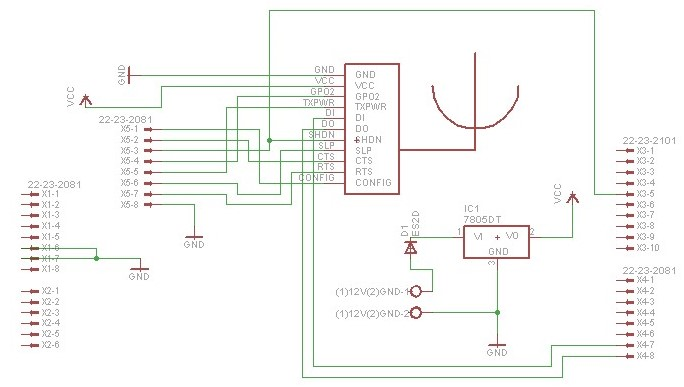
\includegraphics[width=0.9\linewidth]{sch}
\caption{ Displays the schematic of the 9Xtend shield}
\label{sch}
\end{figure}

The shield provides all the correct connections as well as pins for future operations. The shields were designed using Eagle CAD software. A Schematic of the circuit is shown in figure \ref{sch}. From the schematic a board file is generated which displays the physical locations of the module, components of conducting paths. This is displayed in figure \ref{brd}.

\begin{figure}[H]
\centering
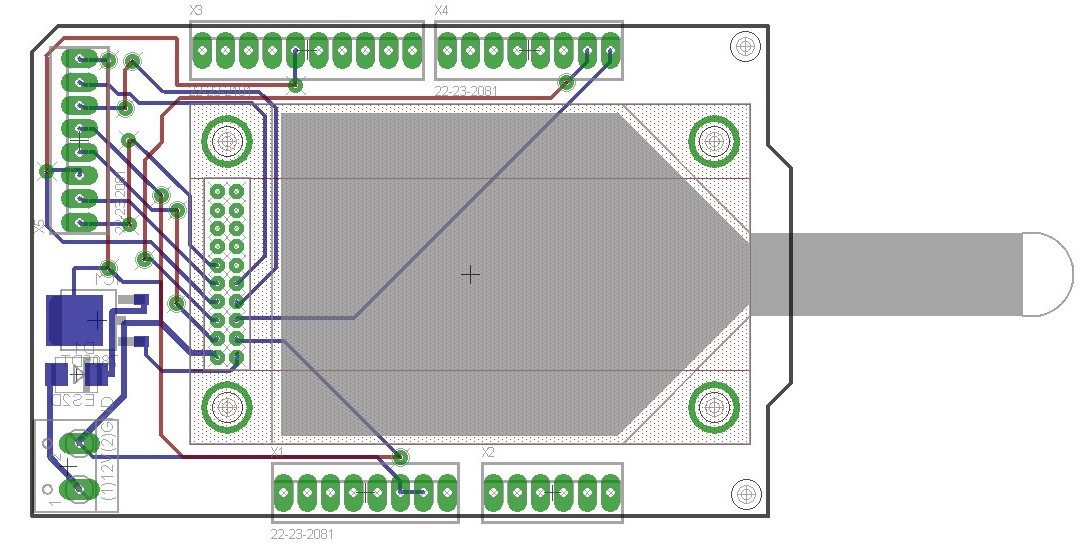
\includegraphics[width=0.9\linewidth]{brd}
\caption{ Displays the board design of the 9Xtend shield}
\label{brd}
\end{figure}

The 9Xtend shield contains accessability to extra pins for future applications. For instance if one wishes to change module settings or switch from transmitting to recieving modes the extra pin set shown in figure \ref{auxi} enables these kinds of operations without having to remove the module or design a new shield.

\begin{figure}[H]
\centering
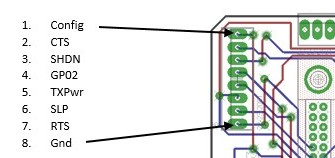
\includegraphics[width=0.75\linewidth]{auxi}
\caption{ Displays the auxiliary inputs/outputs for future functionality}
\label{auxi}
\end{figure}

\section{Arduino Operations}

The Arduino device is an open platform microcontroller. Using a `c' language its functions are easily programmable. A program was created to run on the Arduino with the main purpose of collecting data and outputting to the 9Xtend shield. The programed designed to run with the 9Xtend can read input voltage values, compile them with a string signature, and send them in a UART format to the 9Xtend module. The program also turns off the transmitter during delay times to conserve power. Before a serial string is sent a digital port (pin13) is powered to turn the transmitter on. Data is then transmitted using the serial TX pin. Once transmission is complete the digital pin is reset to low and the module shuts down. The code for the transmitter is displayed in the Appendix, figure \ref{code}. An example of a data string is displayed in figure \ref{string}.The string of data is sent to the module and broadcasted for detection by the receiver.

\begin{figure}[H]
\centering
\normalfont \normalsize \textsc{H681,J289,K423,} \\ [30pt]
\caption{ Displays a typical string transmitted serially. The capital letters are the signature strings.}
\label{string}
\end{figure}

On the receiving module there is a program to find and sort incoming data from the RX line. The commas indicate a stop or space and therefore the reading program will associated the integer number with the preceding signature string. Essentially the receiving program will search for the pre-designated string signatures and once found will read off the valid following integer until a space or comma is found. This integer is then recorded in its corresponding location and thus is distinguished as a particular value from all the other incoming data. This method enables immediate distinction of all the incoming data and therefore is able to record the data in its proper location (example: one location for pressure, one location for temperature..etc). This method also help eliminate invalid data because it requires a specific string and a valid integer to record a data point. If none of these conditions are met the data string is ignored and the program moves on to read the next incoming set. It should be noted that a 500ms delay in the serial string serves the same purpose as a comma and therefore is just as valid. The Arduino code for the receiving module is display in the appendix, figure \ref{code2}.

\section{Testing}
To begin testing its best to ensure the micro-processing units or programs responsible for UART protocol can communicate successfully via a direct serial line. The 9Xtend shields duplicate what is read at the transmitting side to the receiving end. Therefore many problems with communication were easily ruled out with this simple initial test. An example schematic is displayed in figure \ref{test1}.It was very important to have a mutual ground between the two devices, without this communication was problematic.

\begin{figure}[H]
\centering
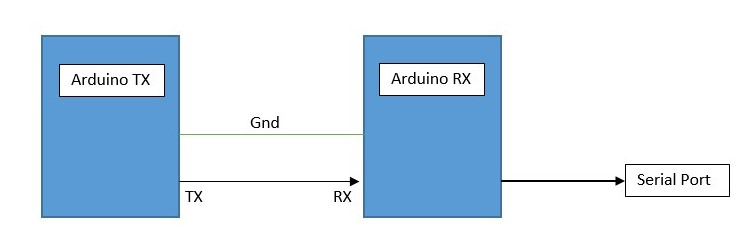
\includegraphics[width=0.9\linewidth]{test1}
\caption{ Displays a typical test to confirm devices communicate using UART protocol}
\label{test1}
\end{figure}

Once the initial UART protocol was mastered the function of the wireless communicators were tested. It was crucial the transmitter and receiver were separated by more than 2m, failing to do so would have resulted in irreversible module damage. The 9Xtend shields were connected as schematically shown in figure \ref{test2}. 

\begin{figure}[H]
\centering
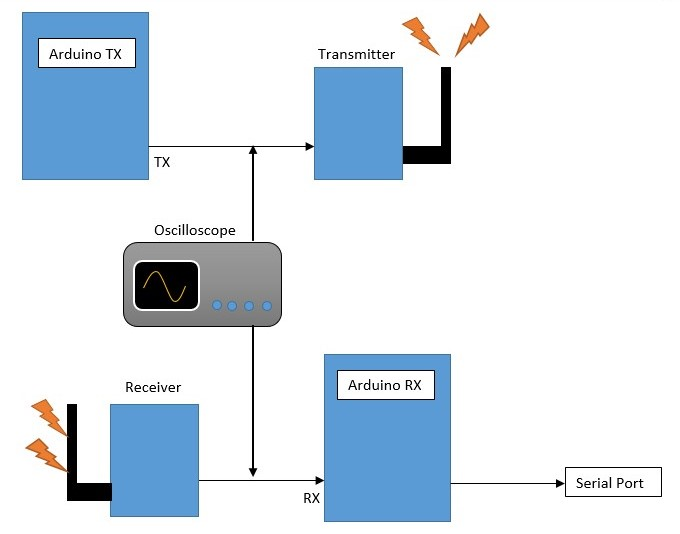
\includegraphics[width=0.9\linewidth]{test2}
\caption{ Displays a typical test to confirm devices communicate using UART protocol}
\label{test2}
\end{figure}

For the transmitter all that was required was inserting the shield on to the Arduino with the correct program. The digital line is already connected to toggle the module. For the receiver when plugged into an Arduino, it is important to make sure the receiving program contains a clip or code to turn pin 13 high. Without this code the module won't turn on and receive. With the serial operations on the Arduino, the UART protocol already sets the input of the module to a high value, therefore throwing it in receiving mode. However if one wishes to use an external device one needs to ensure these conditions are met by pulling the correct auxiliary pins to 5V. More specifically one needs to manually wire, using the auxiliary pins the DI line and SHDN pine of the module to 5V (see Figure \ref{auxi}). This satisfies the UART protocol and ensures the module will be in a receiving mode. Once the transmitter and receiver are operating one can validate the incoming signal by probing the serial connection between the 9Xtend shield and the UART interfacing device

\section{Power Requirements}
The Power requirements for both the transmitter and receiver was experimental validated and is displayed in table \ref{power}. By connecting an ammeter to the input terminals as well as measuring the voltage at the terminal an approximation for power consumption was tabulated.


\begin{table}[H]
\begin{tabularx}{\textwidth}{ |X|X|X|X| }
\hline
Mode & Voltage DC (V) & Current (mA) & Power (W) \\ 
\hline
Transmit & 5 & 725 & 1 \\
\hline
Recieve & 5 & 80& 0.4 \\
\hline
SHDN & 5 & 5uA &0.025mW \\
\hline 
\end{tabularx}
\caption{This table displays the power requirements for the specific modes of operation }
\label{power}
\end{table}




\section{Appendix}


\begin{figure}[H]
\centering
\caption{Displays code programmed for the arduino for transmitting operations}
\label{code}
\end{figure}
\begin{verbatim}
// variables to send over serial
int value1 = 0;
int value2 = 0;
int value3 = 0;
int value4 = 0;
int value5 = 0;
int value6 = 0;

// analog inputs to read
const int analogA0 = A0;
const int analogA1 = A1;
const int analogA2 = A2;
const int analogA3 = A3;
const int analogA4 = A4;
const int analogA5 = A5;

// count is used if want to send data in a burst (reduce data loss) **right now its set to 1
int count = 1;
// sets pin value to D13 on arduino
const int digipin = 13;
//intial value of digital pin is low
int Pintoggle = LOW;

void setup(){
  //sets serial parameters (buad rate 9600), and digital outputs
  pinMode(digipin, OUTPUT);
  digitalWrite(digipin, Pintoggle);
  Serial.begin(9600);
}

void loop(){
  //sets count
  //runs void sendData (reads and transmits data)
  count = 1;
  sendData(value1, value2, value3, value4, value5, value6);
}
\end{verbatim}
\begin{verbatim}
void sendData(int value1, int value2, int value3, int value4, int value5, int value6){
  //  will continue reading and sending until count is zero,***(set to 1 right now) 
  //example every minute could send a burst of 10 data points(if count =10) could eliminate data loss/errors
  while (count > 0){
   // turn on tranismitter by setting pin 13 to high 
   //delay to allow 9Xtend to come out of sleep mode
  Pintoggle = HIGH;
  digitalWrite(digipin, Pintoggle);
  delay(1000); 
  //read analog voltages
  value1 = analogRead(analogA0);
  value2 = analogRead(analogA1);
  value3 = analogRead(analogA2);
  value4 = analogRead(analogA3);
  value5 = analogRead(analogA4);
  value6 = analogRead(analogA5);
  
  //send all values to serial out (TX) 
  // first a string indicater is sent, followed by value then a delay
  Serial.print('H');
  Serial.print(value1);
  delay(500);
  
  Serial.print('J');
  Serial.print(value2);
  delay(500);
  
   Serial.print('K');
  Serial.print(value3);
  delay(500);
  
  Serial.print('L');
  Serial.print(value4);
  delay(500);
  
  Serial.print('M');
  Serial.print(value5);
  delay(500);
  
   Serial.print('I');
  Serial.print(value6);
  delay(500);
  
  // count is decremented, loop ends when zero, 
  //therefore can send a data burst of 5 10... or so times (set to 1 right now)
  count = (count -1);
  }
  //toggle pin 13 back to low to turn transimitter off
  Pintoggle = LOW;
  digitalWrite(digipin, Pintoggle);
  // this is the delay between data transmissions
  delay(2000);
  
 //end of loop
}
\end{verbatim}

\begin{figure}[H]
\centering
\caption{Displays code programmed for the arduino for recieving operations}
\label{code2}
\end{figure}
\begin{verbatim}
int value1, value2, value3 = 0;

void setup(){
  Serial.begin(9600);
}

void loop(){
  value1 = -1;
  value2 = -1;
  readData();
}

void readData(){
  if(Serial.available()){
    
    while (value1 < 100){
    Serial.find("H");
    value1 = Serial.parseInt();
    }
    delay(1000);
    Serial.print("value1:");
    Serial.println(value1);
    
    while (value2 < 100){
    Serial.find("J");
    value2 = Serial.parseInt();
    }
    delay(1000);
    Serial.print("value2:");
    Serial.println(value2);
    
     while (value3 < 100){
    Serial.find("K");
    value2 = Serial.parseInt();
    }
    delay(1000);
    Serial.print("value3:");
    Serial.println(value3); 
}
\end{verbatim}


\begin{thebibliography}{99} % Bibliography - this is intentionally simple in this template
\bibitem[1]{man}
``9Xtend Module Manual'', Digi International Inc. 11001 Bren rd. Minetonka, MN 55343, www.digi.com

\bibitem[2]{picfsk}

http://en.wikipedia.org/wiki/Frequency-shiftkeying

 
\end{thebibliography}
%%% End document
\end{document}